% !TEX root = ../lectures_olympics.tex

\chapter{角动量、力矩和角动量守恒}
\section{有心力作用下的平面运动}
如果一个运动质点的受力的方向永远指向空间中的一个固定点,我们称它受到一个\emph{有心力}的作用,空间中的固定点被称为\emph{力心}。
需要注意的是有心力只与力的方向有关,与力到底是吸引力或排斥力,力的大小是如何变化都没有关系。
对于空间中的一个给定点,将从该点指向运动质点的矢量称为该质点的\emph{矢径}或\emph{向径}。
当质点受到有心力作用时,力的方向永远与矢径的方向相同或相反,而矢径在相同的时间里将扫过相同的面积。
%%%%%%%%%%%%%
\begin{example}
	试从牛顿定律出发证明受到有心力作用下质点的运动将保持在一个平面上,并且相同的时间里矢径扫过相同的面积。
	\tagged{student}{\vspace*{4cm}}
	\begin{taggedblock}{teacher}
		\newline
		解析:略
	\end{taggedblock}
\end{example}
%%%%%%%%%%%%%%%%%%%%



%%%%%%%%%%%%%
\begin{example}
	如果一个运动的质点与空间给定点$O$之间的连线在相同时间里扫过相同的面积,证明它必将受到时刻指向或背离O的力的作用。
	\tagged{student}{\vspace*{4cm}}
	\begin{taggedblock}{teacher}
		\newline
		解析:略
	\end{taggedblock}
\end{example}
%%%%%%%%%%%%%%%%%%%%




\section{力矩,角动量}
有心力作用下的运动满足等面积定律,马上就会想到当外力并不是指向一个固定点时矢径在相同时刻扫过的面积则不是永远相同,本节当中就来研究这种情况。
%%%%%%%%%%%%%%%%%%%%%%%%%%%%%%%%%
\begin{figure}[htbp]
\begin{center}
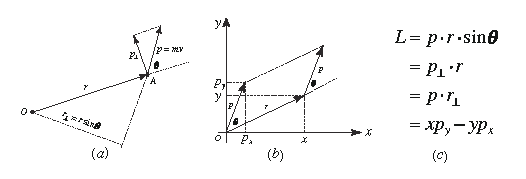
\includegraphics{images/angular-momentum-def-angular-momentum.pdf}
\caption{角动量的不同定义方式,它们对于相同的参考点$O$、相同位置相同速度的质点给出相同的结果}
\label{fig: def of angular momentum}
\end{center}
\end{figure}
%%%%%%%%%%%%%%%%%%%%%%%%%%%%%%%
如图\ref{fig: def of angular momentum}(a)所示,对于一个给定点O,如果一个质量为$m$质点A在某一时刻相对于O的向径为$\vec{r}$,而它的速度用矢量$\vec{v}$给出,定义$\vec{v}$与$\vec{r}$的夹角为$\theta$,那么此时质点P相对于O的角动量被定义为
\begin{equation}
L = p\cdot r\cdot \sin\theta=p_\perp\cdot r = p\cdot r_\perp
\end{equation}
可以将角动量看做是动量在垂直于矢径方向的分量与矢径长度的乘积,或者动量与矢径在垂直于动量方向的投影的乘积。
这样的定有很强的几何意义,如果建立一个以中点$O$为原点的直角坐标系,如图\ref{fig: def of angular momentum}(b)所示当运动质点的位置为$(x,y)$,它动量的分量为$(p_x,p_y)$时,相对于$O$点的角动量同样可以写为
\begin{equation}\label{eqn: 角动量的坐标表达式}
L = xp_y-yp_x.
\end{equation}



%%%%%%%%%%%%%%%%%%%%%
\begin{example}
通过角动量的定义证明\ref{eqn: 角动量的坐标表达式}式。
%\begin{flushright}
%\includegraphics[width = 0.3\textwidth]{images/.pdf} 
%\end{flushright}
\tagged{student}{\vspace*{4cm}}
\begin{taggedblock}{teacher}
\newline
解析:略
\end{taggedblock}
\end{example}
%%%%%%%%%%%%%%%%%%%%%%%}

%%%%%%%%%%%%%%%%%%%%%%%%%%%%%%%%%
\begin{figure}[htbp]
\begin{center}
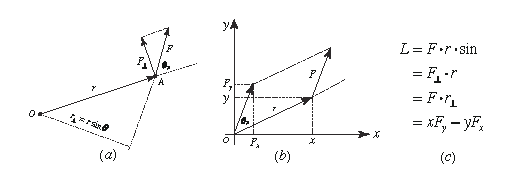
\includegraphics{images/angular-momentum-def-torque.pdf}
\caption{力矩的不同定义方式,和角动量非常相似}
\label{fig: def of torque}
\end{center}
\end{figure}
%%%%%%%%%%%%%%%%%%%%%%%%%%%%%%%
类似地,如图\ref{fig: def of torque}(a)中所示如果前面的质点此时所受的合外力为$\vec{F}$,它受到的相对于O点的力矩
\begin{equation}
M = F r \sin\theta_F = F_\perp\cdot r=F\cdot r_\perp
\end{equation}
其中$\theta_F$为力的方向与矢径方向的夹角。
同样也可在以点$O$为原点的直角坐标系中将力的作用点$A$以及力本身进行正交分解,这时力矩也有类似的分量形式
\begin{equation}\label{eqn: 力矩的分量形式}
M = xF_y - yF_x
\end{equation}

在学习动量时我们知道对于一个质点来说它的动量随时间的变化率等于作用在它上面的外力,与之相类比我们来看角动量对时间的变化率,为此直接计算\ref{eqn: 角动量的坐标表达式}式对时间的变化率:
\begin{eqnarray*}
\frac{\Delta L}{\dt}&=&\frac{\Delta (xp_y)}{\dt}-\frac{\Delta (yp_x)}{\dt} = \frac{\Delta x}{\dt}p_y+x\frac{\Delta p_y}{\dt}-\frac{\Delta y}{\dt}p_x+y\frac{\Delta p_x}{\dt}\\
&=& v_x p_y+xF_y-v_yp_x-yp_x = xF_y-yF_x = M
\end{eqnarray*}
可以看出角动量随时间的变化率不是别的,正是此时作用于质点的合外力对同样的中点$O$产生的力矩的大小,这个事实可以看做是牛顿定律对于角运动的推广:
\begin{equation}\label{eqn: 角动量定律}
M = \frac{\Delta L}{\dt}.
\end{equation}

对于作用时间极短的冲击过程,可以定义质点受到的冲量在垂直于矢径的方向的分量与矢径大小的乘积
\begin{equation}
J = I_\perp r
\end{equation}
为质点所受到的\emph{冲量矩},动量定理可以推广到角运动的情况:质点受到的冲量矩等于角动量的变化量:
\begin{equation}
J = \Delta L
\end{equation}

%%%%%%%%%%%%%%%%%%%%%%%%%%%%%
\section{角动量守恒定律}

从角动量定理可以看出,当一个质点所受力矩为零时它的角动量随时间的变化率为零,也就是说角动量不随时间而变,我们称此时运动质点\emph{角动量守恒}。
有心力与矢径夹角的正弦永远为零,所以无论有心力的大小如何变化它们对于力心的力矩必然为零,所以仅在有心力作用下运动的物体相对于力心的角动量必然守恒。




\begin{example}
有心力作用下矢径在单位时间里扫过的面积为常数,现在我们又知道有心力作用下的角动量也是常数,可以料想它们之间必然有着某种关联,尝试找出矢径的面积速度与角动量的关系。
%\begin{flushright}
%\includegraphics[width = 0.3\textwidth]{images/.pdf} 
%\end{flushright}
\tagged{student}{\vspace*{4cm}}
\begin{taggedblock}{teacher}
\newline
解析:略
\end{taggedblock}
\end{example}




\begin{example}
判断角动量是否守恒:

(1)光滑平面上由系在弹簧上的球相对于固定弹簧的点,假设在运动过程中弹簧始终保持直线。

(2)粗糙平面上由系在弹簧上的球相对于固定弹簧的点,假设在运动过程中弹簧始终保持直线。

(3)光滑平面上由系在弹簧上的球相对于固定弹簧的点,但在运动过程中弹簧有可能弯曲。

(4)竖直悬挂的弹簧上的质点相对于固定弹簧的点。

(5)抛出的物体相对于地面某点。

(6)抛出的物体相对于地心。
%\begin{flushright}
%\includegraphics[width = 0.3\textwidth]{images/.pdf} 
%\end{flushright}
\tagged{student}{\vspace*{4cm}}
\begin{taggedblock}{teacher}
\newline
解析:是是否是否是
\end{taggedblock}
\end{example}

在有心力作用下运动质点的速度可以分解为径向和横向分量,当径向速度为零时它必然处在与力心距离的最大值或最小值处。
这时质点的运动速度与矢径垂直,它的角动量自然就是其横向动量与距离力心距离的乘积。
与力心距离的极值具有非常重要的理论和现实意义,如果向心力同时为保守力时根据机械能守恒和角动量守恒可以在某些情况下求出运动质点与力心距离的极值。





\begin{example}
光滑水平面有一根一端固定在$O$点原长为零、弹性系数为$k$、不计自重的弹簧。
初始时刻一个质量为$m$的质点固定在弹簧的另一端,距离$O$点$r_0$,以垂直于弹簧的初速度$v_0$被发射出去。
求该质点在此后运动中与$O$的最大和最小距离。
%\begin{flushright}
%\includegraphics[width = 0.3\textwidth]{images/.pdf} 
%\end{flushright}
\tagged{student}{\vspace*{4cm}}
\begin{taggedblock}{teacher}
\newline
解析:角动量守恒和能量守恒,列出两个方程式,会有两个解,分别为最大距离和最小距离的解,题目里面给出的初始条件是解之一。
\[mv_0r_0=mv_1r_1\]
\[\frac{1}{2}mv_1^2+\frac{1}{2}kr_1^2=\frac{1}{2}mv_0^2+\frac{1}{2}kr_0^2\]
解出的另外一个解:\[r_1=\sqrt{\frac{m}{k}}v_0\]
\end{taggedblock}
\end{example}

\begin{example}
空间中有一固定点$O$,一质量为$m$的质点在以$O$为中心的有心力场中运动,该力为保守力,其势函数由$E_p(r)=-\frac{A}{r}$给出,由此可知该质点的机械能$E=(\frac{1}{2}mv^2-\frac{A}{r})$守恒。
当该质点距离力心$r_0$时具有垂直于与力心的连线的速度$v_0$,求在此后的运动过程中它与中心$O$点的最大和最小距离。
%\begin{flushright}
%\includegraphics[width = 0.3\textwidth]{images/.pdf} 
%\end{flushright}
\tagged{student}{\vspace*{4cm}}
\begin{taggedblock}{teacher}
\newline
解析:角动量守恒和能量守恒,列出两个方程式,会有两个解,分别为最大距离和最小距离的解,题目里面给出的初始条件是解之一。
\[mv_0r_0=mv_1r_1\]
\[\frac{1}{2}mv_1^2-\frac{A}{r_1}=\frac{1}{2}mv_0^2-\frac{A}{r_0}\]
解出:\[\frac{1}{r}=\frac{A}{mv_0^2r_0^2}\pm(\frac{A}{mv_0^2r_0^2}-\frac{1}{r_0})\]
\end{taggedblock}
\end{example}


\begin{example}
在和上题一样的力心为$O$的有心力作用下,一个质量为$m$的质点由无限远处以速度$v_0$运动。
$O$点与它的速度方向的延长线的最短距离为$b$,求在此后的运动过程中它与中心$O$点的最小距离。
%\begin{flushright}
%\includegraphics[width = 0.3\textwidth]{images/.pdf} 
%\end{flushright}
	\begin{flushright}
		\includegraphics[width = 0.4\textwidth]{images/ang-momontum-4.pdf} 
	\end{flushright}
\tagged{student}{\vspace*{4cm}}
\begin{taggedblock}{teacher}
\noindent
解析:\[mvr=mv_0b\]
\[\frac{1}{2}mv^2-\frac{A}{r}=\frac{1}{2}mv^0\]
解出:\[\frac{1}{r}=\frac{A}{mv_0^2b^2}+\sqrt{(\frac{A}{mv_0^2b^2})^2+\frac{1}{b^2}}\]
\end{taggedblock}
\end{example}

%\begin{example}
%如果一个质量为$m$的质点始终受到一个指固定点$O$保守的有心力的作用,在该保守力下的势能$E_p = -\frac{A}{r^4}$,初始时刻它距离$O$无限远处以速度$v_0$向着$O$运动,$O$与其初速度延长线方向的垂线距离为$b$,如果要求它不能够逃离$O$点的吸引力,那么$b$所允许的最大值为多少?
%\begin{flushright}
%\includegraphics[width = 0.3\textwidth]{images/.pdf} 
%\end{flushright}
%\tagged{student}{\vspace*{4cm}}
%\begin{taggedblock}{teacher}
%\newline
%解析:
%\end{taggedblock}
%\end{example}


%%%%%%%%%%%%%%%%%%%%%%%%%%%%%%%%%
\begin{figure}[htbp]
	\begin{center}
		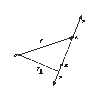
\includegraphics[width=0.4\textwidth]{images/angular-momentum-angular-conservation-many.pdf}
		\caption{系统内部质点之间的相互作用力的力矩大小相等、方向相反}
		\label{fig: 系统内部质点之间的相互作用力的力矩大小相等、方向相反}
	\end{center}
\end{figure}
%%%%%%%%%%%%%%%%%%%%%%%%%%%%%%%
\section{质点系统的角动量守恒}
当将多个质点看做一个力学系统时,该力学系统相对于给定的中心点的角动量自然就是系统内部所有质点相对同一点的角动量之和。
和动量守恒的情况类似,当整个系统不受任何外力作用,或者外力相对于中心点的力矩为零时,整个系统的角动量守恒。
如图\ref{fig: 系统内部质点之间的相互作用力的力矩大小相等、方向相反}所示,根据牛顿第三定律由内力所产生的不同质点上的力矩大小相等方向相反,彼此抵消了。




%\begin{example}
%判断以下各种情况中相对给定点的角动量是否守恒:
%
%(1)太阳系中所有天体在引力作用下以太阳或太阳系全部物质质心为中心的角动量
%
%(2)地球和月球构成的系统对地心的角动量,地月系统相对于地月系心的角动量
%
%(3)光滑轴对称平面内运动的质点相对于轴线的角动量。
%
%(4)竖直平面上一端系在固定点,一端系有重物的系统。
%
%(5)光滑水平桌面上无质量的绳子两端系有两个物体相对于任意一点的角动量。
%\end{example}


\begin{example}
轻杆可以围绕固定点$O$自由无阻力转动,质量为$2m$的$A$球开始固定在轻杆的中点,质量为$m$的B球固定在杆的下方端点处。
一个质量也为$m$的球$C$以速度$v$入射,之后与$B$发生完全非弹性碰撞。
求合体后的一瞬间$A$的速度多大?
如果碰撞为完全弹性碰撞,此时$A$的速度又是多少?
	\begin{flushright}
		\includegraphics[width = 0.2\textwidth]{images/ang-momontum-3.pdf} 
	\end{flushright}
	\tagged{student}{\vspace*{4cm}}
\begin{taggedblock}{teacher}
\noindent
解析:角动量守恒、能量不守恒$v_A=\frac{v_0}{5}$
\\
角动量守恒、能量守恒$v_A=\frac{2v_0}{5}$
\end{taggedblock}
\end{example}




\begin{example}
在水平桌面上有一个轻刚性杆两端分别有一个质量为$m_{1}$,$m_2$的质点,另一个质量为$m_3$的质点以速度$v_0$以垂直于杆的方向与A发生完全弹性碰撞,求碰撞之后各个质点的速度各是多少?
	\begin{flushright}
		\includegraphics[width = 0.3\textwidth]{images/ang-momontum-2.pdf} 
	\end{flushright}
	\tagged{student}{\vspace*{4cm}}
\begin{taggedblock}{teacher}
\noindent
解析:角动量守恒,$m_2$不会动,于是结果就是1球与3球发生完全弹性碰撞,
$v_3=\frac{m_3-m_2}{m_3+m_2}v_0$   $v_1=\frac{2m_3}{m_2+m_3}v_0$  
\end{taggedblock}
\end{example}



\begin{example}
在水平桌面上有一个轻刚性杆,其两端的中心处有三个质量同为$m$的质点,另一个质量为$m_3$的质点以速度$v_0$以垂直于杆的方向与A发生完全非弹性碰撞,求碰撞之后各个质点的速度各是多少?
	\begin{flushright}
		\includegraphics[width = 0.3\textwidth]{images/ang-momontum-1.pdf} 
	\end{flushright}
	\tagged{student}{\vspace*{4cm}}
\begin{taggedblock}{teacher}
\noindent
解析:碰撞之后三个球都会动,质心会有一个速度,然后三个球在质心参考系中围着质心转动。因为是完全非弹性碰撞,所以能量不守恒,但是动量和角动量守恒。而且是以任何点为参考的角动量都守恒。根据角动量守恒,动量守恒,几何关系,就可以解题了。以$v_0$方向为正方向。
最左:$\frac{5m_3}{6m+5m_3}$中间:$\frac{2m_3}{6m+5m_3}$最右:$\frac{-m_3}{6m+5m_3}$
\end{taggedblock}
\end{example}





